\documentclass[12pt, answers]{exam}
%\documentclass[12pt]{exam}
%\setlength{\textheight}{5in}
%\usepackage[textwidth=9in,centering]{geometry}
\usepackage[a4paper, margin=1in]{geometry}
\usepackage{econometrics}
\usepackage{lmodern}
\usepackage{amssymb,amsmath,amsfonts,amsthm,enumerate,enumitem}
\usepackage{setspace, graphicx, multirow, dcolumn, caption}
\usepackage{bm, booktabs}
\pagestyle{empty}

\firstpagefooter{}{Page \thepage\ of \numpages}{}
\runningfooter{}{Page \thepage\ of \numpages}{}

% \usepackage{etoolbox}
% \AtEndEnvironment{question}{\bigskip\bigskip}

% \usepackage{etoolbox}
% \makeatletter
%  \patchcmd\@setheadheight{\endgroup}{\global\vsize=\textheight\endgroup}{}{}
% \makeatother


% Notation
\def\eps{\varepsilon}
\def\var{\text{Var}}
\def\cov{\text{Cov}}
\def\corr{\text{Corr}}
\def\Ybar{\overline{Y}}
\def\Xbar{\overline{X}}
\def\ybar{\overline{y}}
\def\xbar{\overline{x}}
\def\Yhat{\widehat{Y}}
\def\yhat{\widehat{y}}
\def\fhat{\widehat{f}}
\def\bhat{\widehat{\beta}}
\def\betahat{\widehat{\vbeta}}
\def\MSE{\text{MSE}}
\def\SE{\text{SE}}
\def\train{\mathcal{T}}
\def\data{\mathcal{D}}
\def\model{\mathcal{M}}
\def\hvtheta{\widehat{\vtheta}}
\def\({\left(}
\def\){\right)}



\makeatletter
\g@addto@macro\@floatboxreset\centering
\makeatother



\setlength{\parindent}{0pt}
\onehalfspace

%\renewcommand{\labelitemi}{1.}

%\bracketedpoints
\pointpoints{mark}{marks}
% \qformat{\textbf{Problem \thequestion: \\ \hspace{10pt} \\}}


\qformat{
    \textbf{Question \thequestion \hspace{2pt} \thepoints}
    \hfill
    \vrule depth 20pt width 0pt % Large depth to make space
}

\bonusqformat
{
    \textbf{Question \thequestion \hspace{2pt} \thepoints}
    \hfill
    \vrule depth 20pt width 0pt % Large depth to make space
}

\bonuspointpoints{mark, bonus)}{marks, bonus}


\begin{document}



\begin{center}
{\Large \textbf{QBUS6810} \\\textbf{Statistical Learning and Data Mining}}\\  \large{Tutorial 13 (Solutions)}
\end{center}




\begin{questions}

\question

Suppose that you want to train a Naive Bayes classifier for the following data.

\smallskip

\begin{center}
\begin{tabular}{ll|l}
\toprule
\multicolumn{2}{c}{\textbf{Inputs}}      &          \multicolumn{1}{c}{\textbf{Output}}   \\
\multicolumn{1}{c}{Salary ($X_1$)} & \multicolumn{1}{c}{Spouse Salary ($X_2$)} & \multicolumn{1}{c}{Happy (H)}\\ \midrule
80          & 60         & Yes ($1$)    \\
100          & 80         & Yes ($1$)    \\
70          & 80   & No ($0$)   \\
50          & 20   & No ($0$)   \\ \bottomrule
\end{tabular}
\end{center}

\smallskip

The unit of measurement for Salary is \$1K.

\smallskip

\begin{parts}

\part Assume that the distribution of Salary given the value of H is Gaussian, i.e. the class conditional densities for $X_1$ are:
\begin{align*}
p(x_1|H=h)=\frac{1}{\sqrt{2\pi\sigma^2_{1h}}}\exp\left(-\frac{\(x_1-\mu_{1h}\)^2}{2\sigma^2_{1h}}\right),\quad \text{for}\; h=0\;\text{and}\; h=1.
\end{align*}
Estimate (using the data) the means $\mu_{1h}$ and the variances $\sigma^2_{1h}$ for $h=0$ and $h=1$.  Show your work.

\begin{solution}
The class conditional mean and variance are estimated by maximum likelihood.  As we are assuming the class conditional distribution is Gaussian, the resulting estimate of the mean is simply the average Salary within the class, while the resulting estimate of the variance is the average squared deviation from the estimated mean.

\begin{align*}
&H=0\; \text{(unhappy class):}\\[4pt]
\widehat{\mu}_{10}&=\frac{70+50}{2}=60\\[2pt]
\widehat{\sigma}^2_{10}&=\frac{(70-60)^2+(50-60)^2}{2}=100\\
\\
&H=1\; \text{(happy class):}\\[4pt]
\widehat{\mu}_{11}&=\frac{80+100}{2}=90\\[2pt]
\widehat{\sigma}^2_{11}&=\frac{(80-90)^2+(100-90)^2}{2}=100\\
\end{align*}
\end{solution}


\part Assume that the distribution of the Spouse Salary given the value of H is also Gaussian, i.e. the class conditional densities for $X_2$ are:
\begin{align*}
p(x_2|H=h)=\frac{1}{\sqrt{2\pi\sigma^2_{2h}}}\exp\left(-\frac{\(x_1-\mu_{2h}\)^2}{2\sigma^2_{2h}}\right),\quad \text{for}\; h=0\;\text{and}\; h=1.
\end{align*}
Estimate the means $\mu_{2h}$ and the variances $\sigma^2_{2h}$ for $h=0$ and $h=1$.

\begin{solution}
This is analogous to the previous part.  The estimate of the mean is simply the average Spouse Salary within the class, while the estimate of the variance is the average squared deviation from the estimated mean.
\begin{align*}
&H=0\; \text{(unhappy class):}\\[4pt]
\widehat{\mu}_{20}&=\frac{80+20}{2}=50\\[2pt]
\widehat{\sigma}^2_{20}&=\frac{(80-50)^2+(20-50)^2}{2}=900\\
\\
&H=1\; (\text{(happy class):}\\[4pt]
\widehat{\mu}_{21}&=\frac{60+80}{2}=70\\[2pt]
\widehat{\sigma}^2_{21}&=\frac{(60-70)^2+(80-70)^2}{2}=100\\
\end{align*}
\end{solution}

\bigskip


\part Estimate  (using the data) the class probabilities: $P(H=1)$ and $P(H=0)$.


\begin{solution}

The maximum likelihood estimates of the class probabilities are simply the class proportions:
\begin{align*}
\widehat{P}(H=1)&=\frac{2}{4}=0.5\\[2pt]
\widehat{P}(H=0)&=\frac{2}{4}=0.5 \;\; = \;\; 1-\widehat{P}(H=1).
\end{align*}

\end{solution}

\bigskip

\part Derive the Naive Bayes classifier estimate of the probability\\ $P(H=1|X_1=x_1,X_2=x_2)$, first using the general formulas, and then incorporating your specific results from parts (a), (b), and (c).


\begin{solution}

To simplify the notation, define $\pi_1=P(H=1)$ and $\pi_0=P(H=0)$.  From part (b) we have $\widehat{\pi}_1=0.5=\widehat{\pi}_0$.

\bigskip



The Naive Bayes classifier makes the critical assumption that the predictors ($X_1$ and $X_2$) are independent conditional on the class. Using Bayes' theorem, the probability that an individual is happy conditional on $X_1$ and $X_2$ is

\begin{align*}
&P(H=1|X_1=x_1, X_2=x_2)\;=\\
\\
&\frac{\pi_1\, p(x_1|H=1)p(x_2|H=1)}{\pi_1\, p(x_1|H=1)p(x_2|H=1)+\pi_0\,p(x_1|H=0)p(x_2|H=0)}
\end{align*}


\bigskip

In the Naive Bayes method, we estimate $\pi_0, \pi_1$, and the parameters of the class conditional densities as in the previous three parts of the question.   We then compute the estimated conditional probability:
\begin{align*}
&\widehat{P}(H=1|X_1=x_1, X_2=x_2)\;=\\
\\
&\frac{\widehat{\pi}_1\, \widehat{p}(x_1|H=1)\widehat{p}(x_2|H=1)}{\widehat{\pi}_1\, \widehat{p}(x_1|H=1)\widehat{p}(x_2|H=1)+\widehat{\pi}_0\,\widehat{p}(x_1|H=0)\widehat{p}(x_2|H=0)}.
\end{align*}

\bigskip

Recall that $\widehat{\pi}_1=0.5=\widehat{\pi}_0$, and the estimated class conditional densities are:

\bigskip
\begin{align*}
\widehat{p}(x_1|H=0)&= \frac{1}{\sqrt{2\pi\widehat{\sigma}^2_{10}}}\exp\left(-\frac{\(x_1-\widehat{\mu}_{10}\)^2}{2\widehat{\sigma}^2_{10}}\right)
=\frac{1}{\sqrt{2\pi\times100}}\exp\left(-\frac{\(x_1-60\)^2}{2\times100}\right)
\end{align*}
\begin{align*}
\widehat{p}(x_1|H=1)&= \frac{1}{\sqrt{2\pi\widehat{\sigma}^2_{11}}}\exp\left(-\frac{\(x_1-\widehat{\mu}_{11}\)^2}{2\widehat{\sigma}^2_{11}}\right)
=\frac{1}{\sqrt{2\pi\times100}}\exp\left(-\frac{\(x_1-90\)^2}{2\times100}\right)
\end{align*}
\begin{align*}
\widehat{p}(x_2|H=0)&= \frac{1}{\sqrt{2\pi\widehat{\sigma}^2_{20}}}\exp\left(-\frac{\(x_2-\widehat{\mu}_{20}\)^2}{2\widehat{\sigma}^2_{20}}\right)
=\frac{1}{\sqrt{2\pi\times900}}\exp\left(-\frac{\(x_2-50\)^2}{2\times900}\right)
\end{align*}
\begin{align*}
\widehat{p}(x_2|H=1)&= \frac{1}{\sqrt{2\pi\widehat{\sigma}^2_{21}}}\exp\left(-\frac{\(x_2-\widehat{\mu}_{21}\)^2}{2\widehat{\sigma}^2_{21}}\right)
=\frac{1}{\sqrt{2\pi\times100}}\exp\left(-\frac{\(x_2-70\)^2}{2\times100}\right)
\end{align*}

\medskip

Putting it all together, the \textbf{numerator} of $\widehat{P}(H=1|X_1=x_1, X_2=x_2)$ is
\begin{equation*}
{0.5\times \frac{1}{\sqrt{2\pi\times100}}\exp\left(-\frac{\(x_1-90\)^2}{2\times100}\right) \times \frac{1}{\sqrt{2\pi\times100}}\exp\left(-\frac{\(x_2-70\)^2}{2\times100}\right)}
\end{equation*}
and the \textbf{denominator} is
\begin{align*}
&0.5\times \frac{1}{\sqrt{2\pi\times100}}\exp\left(-\frac{\(x_1-90\)^2}{2\times100}\right) \times \frac{1}{\sqrt{2\pi\times100}}\exp\left(-\frac{\(x_2-70\)^2}{2\times100}\right)\\
\\
&+\;0.5\times \frac{1}{\sqrt{2\pi\times100}}\exp\left(-\frac{\(x_1-60\)^2}{2\times100}\right) \times \frac{1}{\sqrt{2\pi\times900}}\exp\left(-\frac{\(x_2-50\)^2}{2\times900}\right).
\end{align*}

\bigskip

After cancelling out various constants we derive:
\begin{align*}
&\widehat{P}(H=1|X_1=x_1, X_2=x_2)\;=\\
\\
&\frac{\exp\left(-\frac{\(x_1-90\)^2+\(x_2-70\)^2}{200}\right)}
{\exp\left(-\frac{\(x_1-90\)^2+\(x_2-70\)^2}{200}\right)+
\frac{1}{3}\exp\left(-\frac{\(x_1-60\)^2}{200}-\frac{\(x_2-50\)^2}{1800}\right)}.
\end{align*}

Given an individual with Salary $x_1$ and Spouse Salary $x_2$, we will classify that individual as happy if the above probability is greater than $0.5$.

\end{solution}


\end{parts}

\clearpage


\question

Suppose $X_1$ and $X_2$ take values in the interval $[0,10]$.

\begin{parts}

\part

Consider the following regression tree.  The numbers next to the terminal nodes give the corresponding predicted values.

\begin{figure}[!ht]
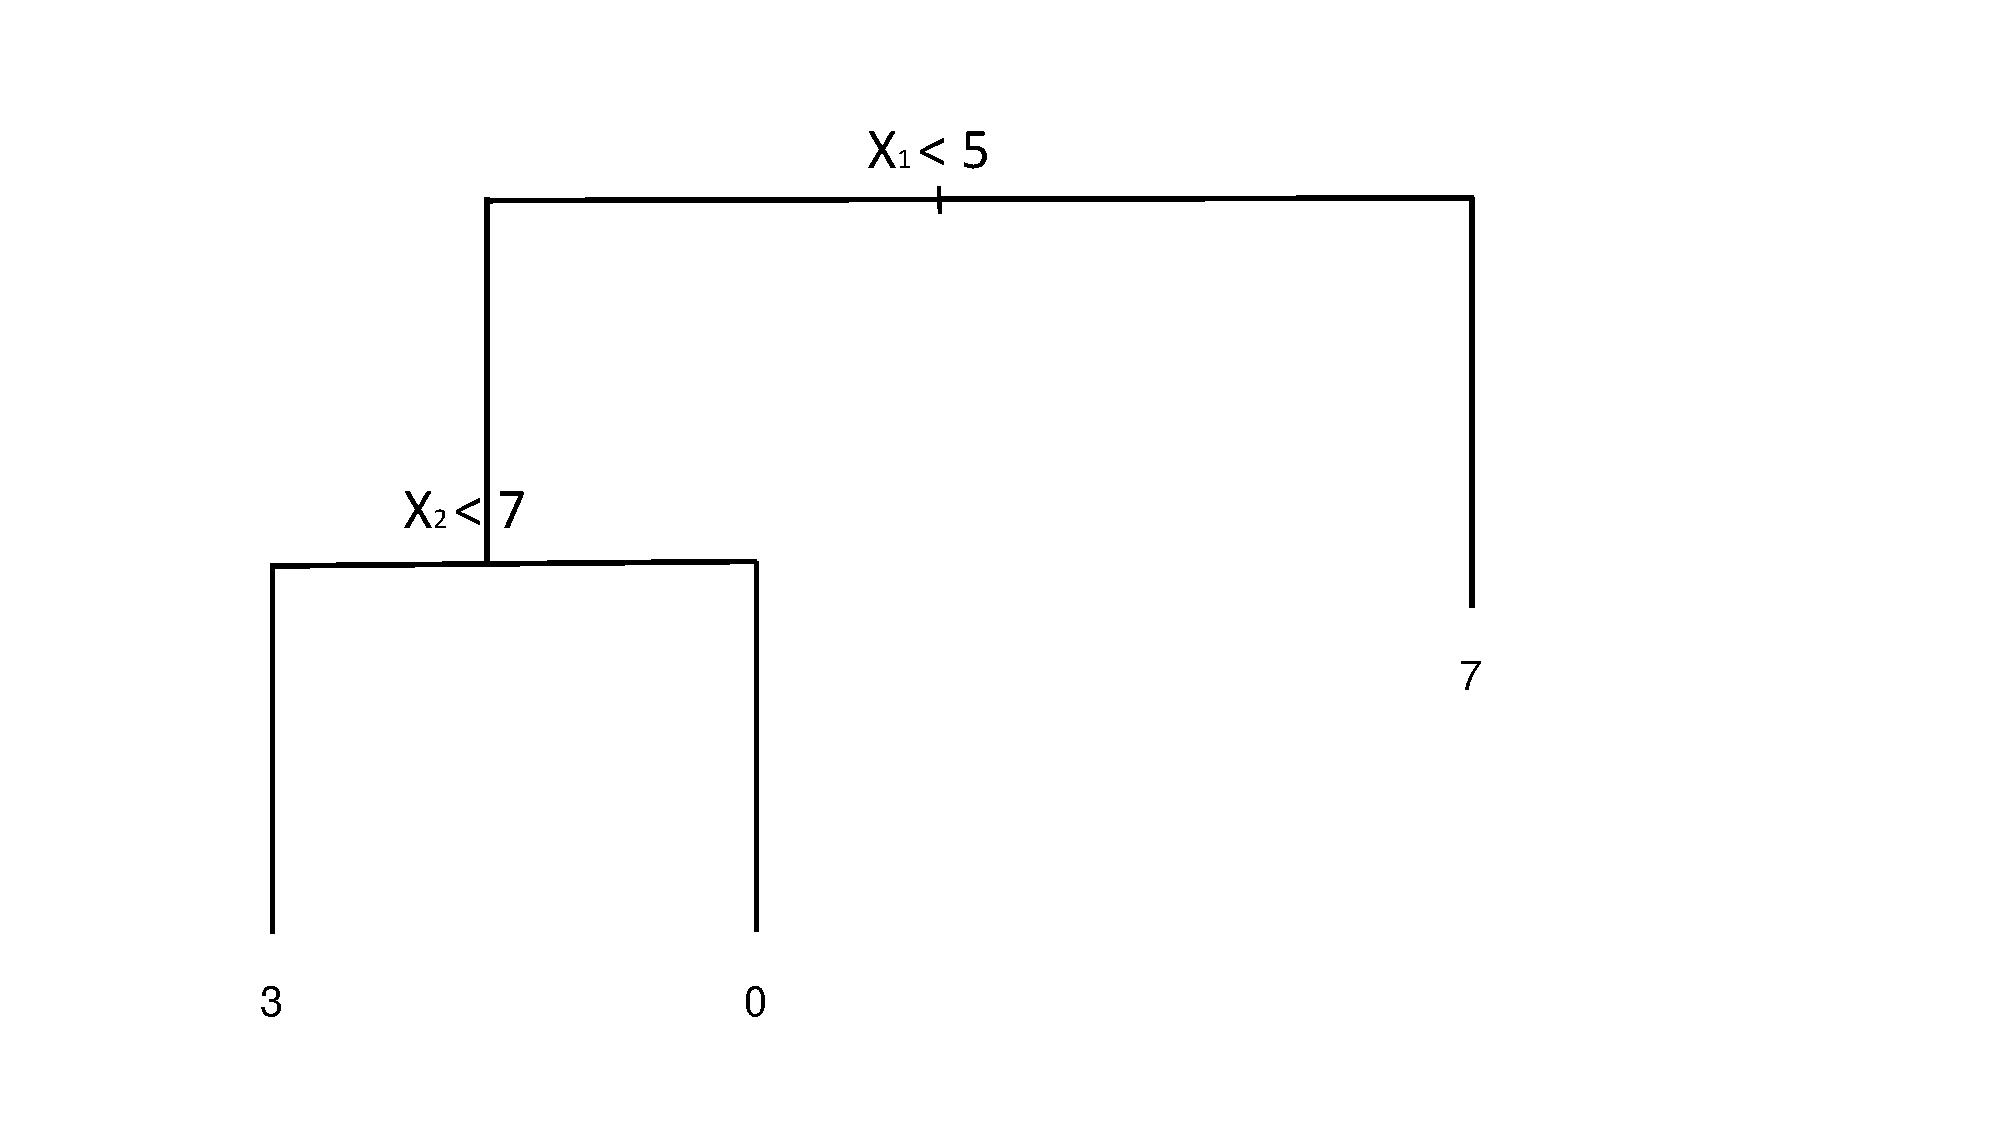
\includegraphics[scale=0.4]{T1.pdf}
\end{figure}

Sketch the corresponding partition of the predictor space.  Write the predicted values inside the corresponding regions of the partition.

\part

Now consider the following partition of the predictor space.

\begin{figure}[!ht]
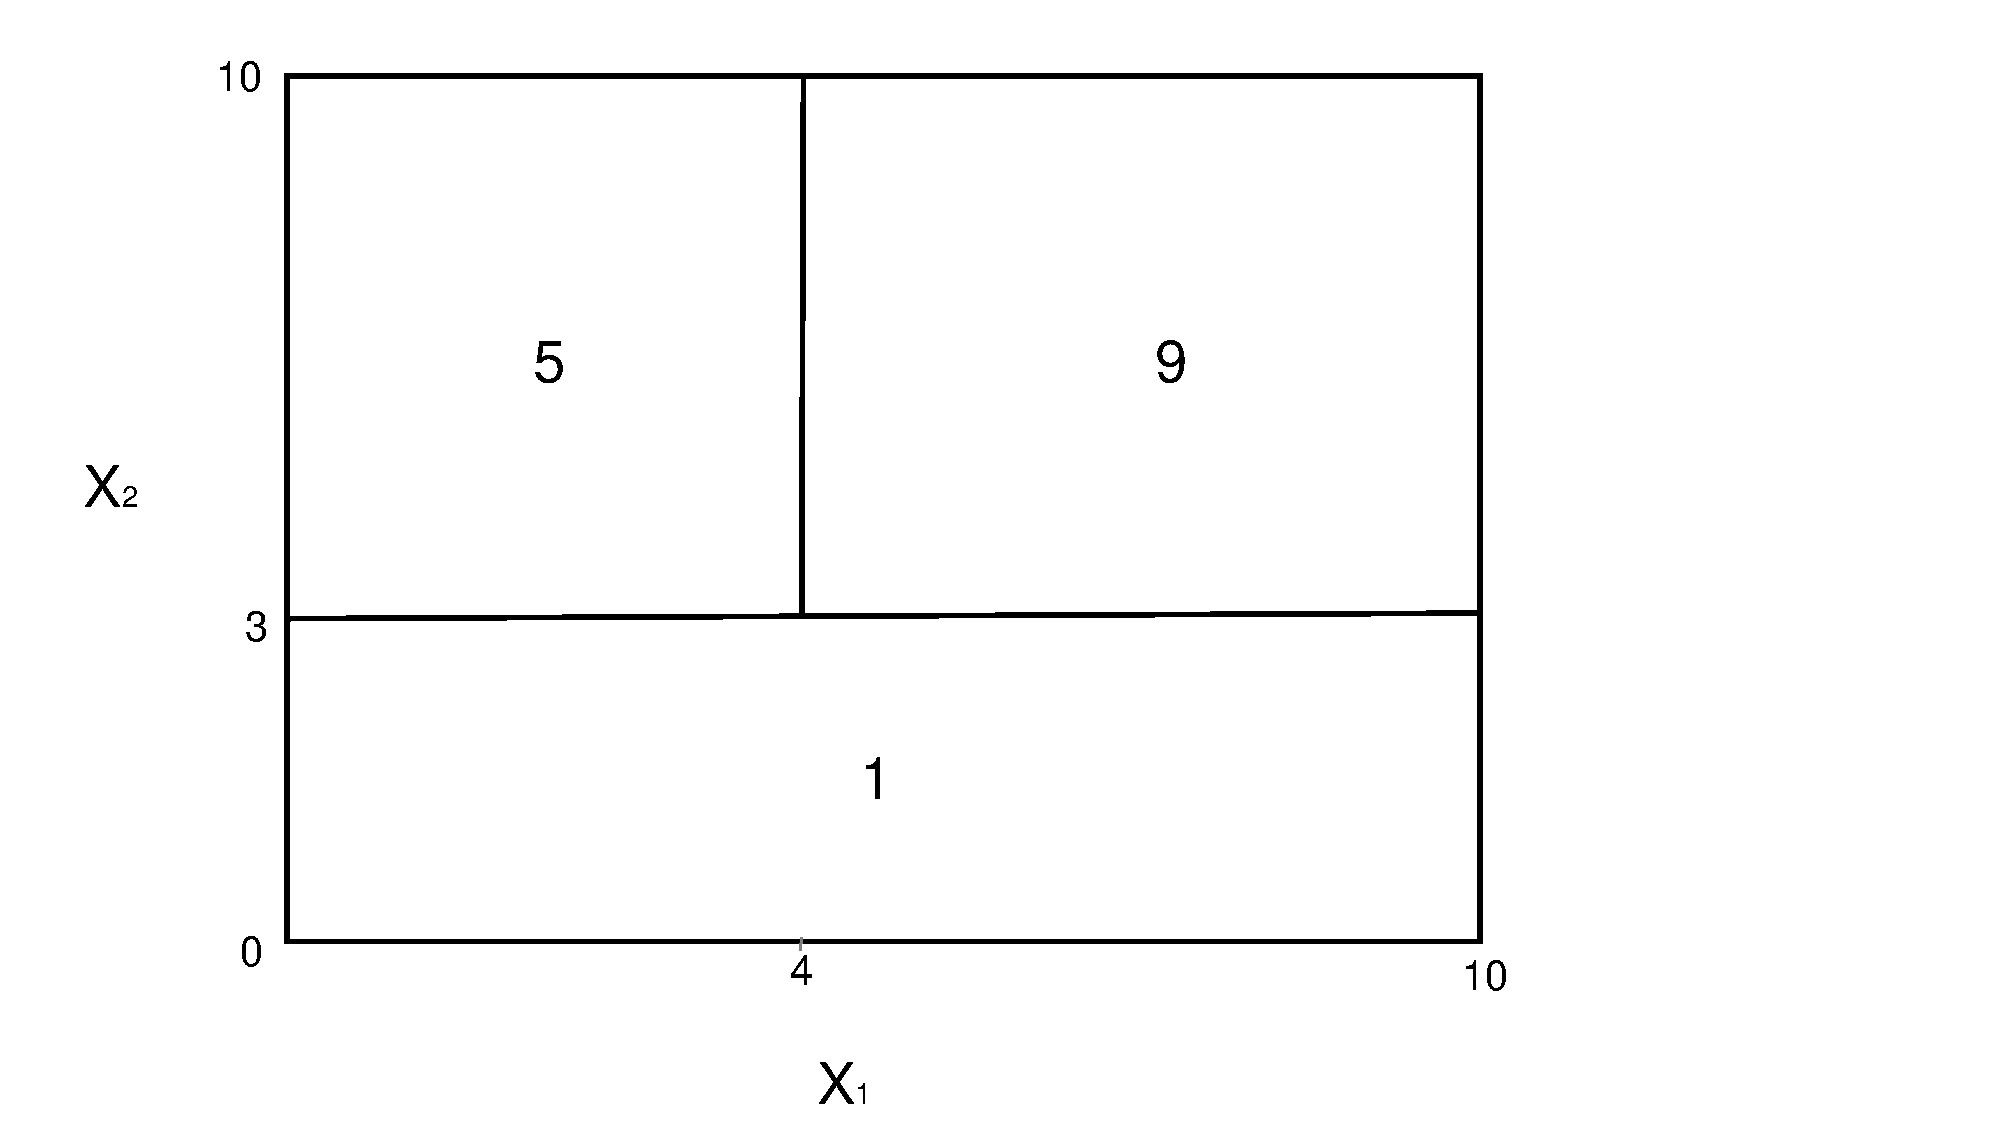
\includegraphics[scale=0.4]{P2.pdf}
\end{figure}

Create a diagram for the corresponding regression tree.

\part For the tree in part b), write down the estimated regression function, $\widehat{f}(x_1,x_2)$.  Does this function correspond to a GAM (i.e. an additive model) or a model with interactions?

\end{parts}

\end{questions}


\textbf{Solution.}


\textbf{(a)} \textit{We start with the entire predictor space:}

\begin{figure}[!ht]
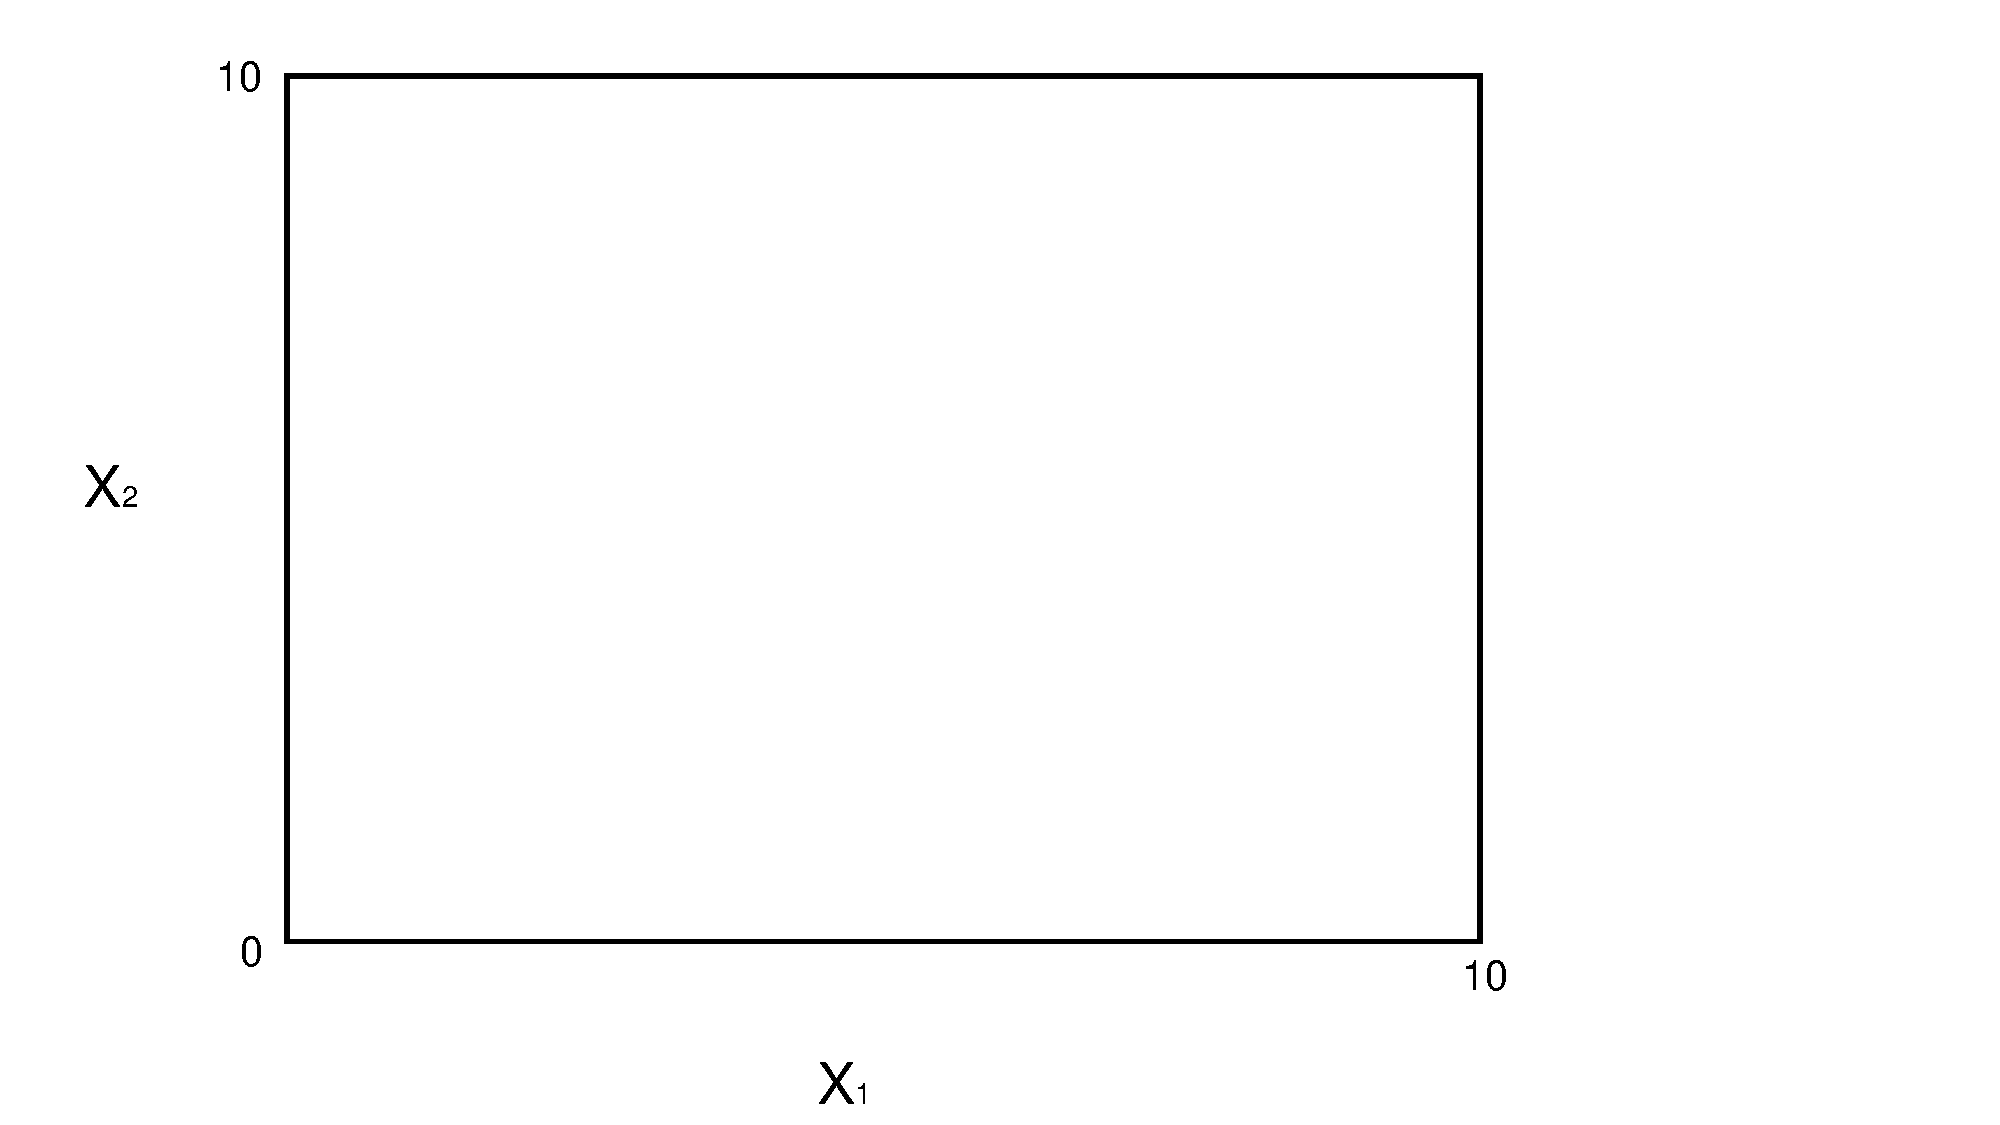
\includegraphics[scale=0.22]{P1a.pdf}
\end{figure}

\textit{The first split, $X_1<5$, results in the following partition:}
\begin{figure}[!h]
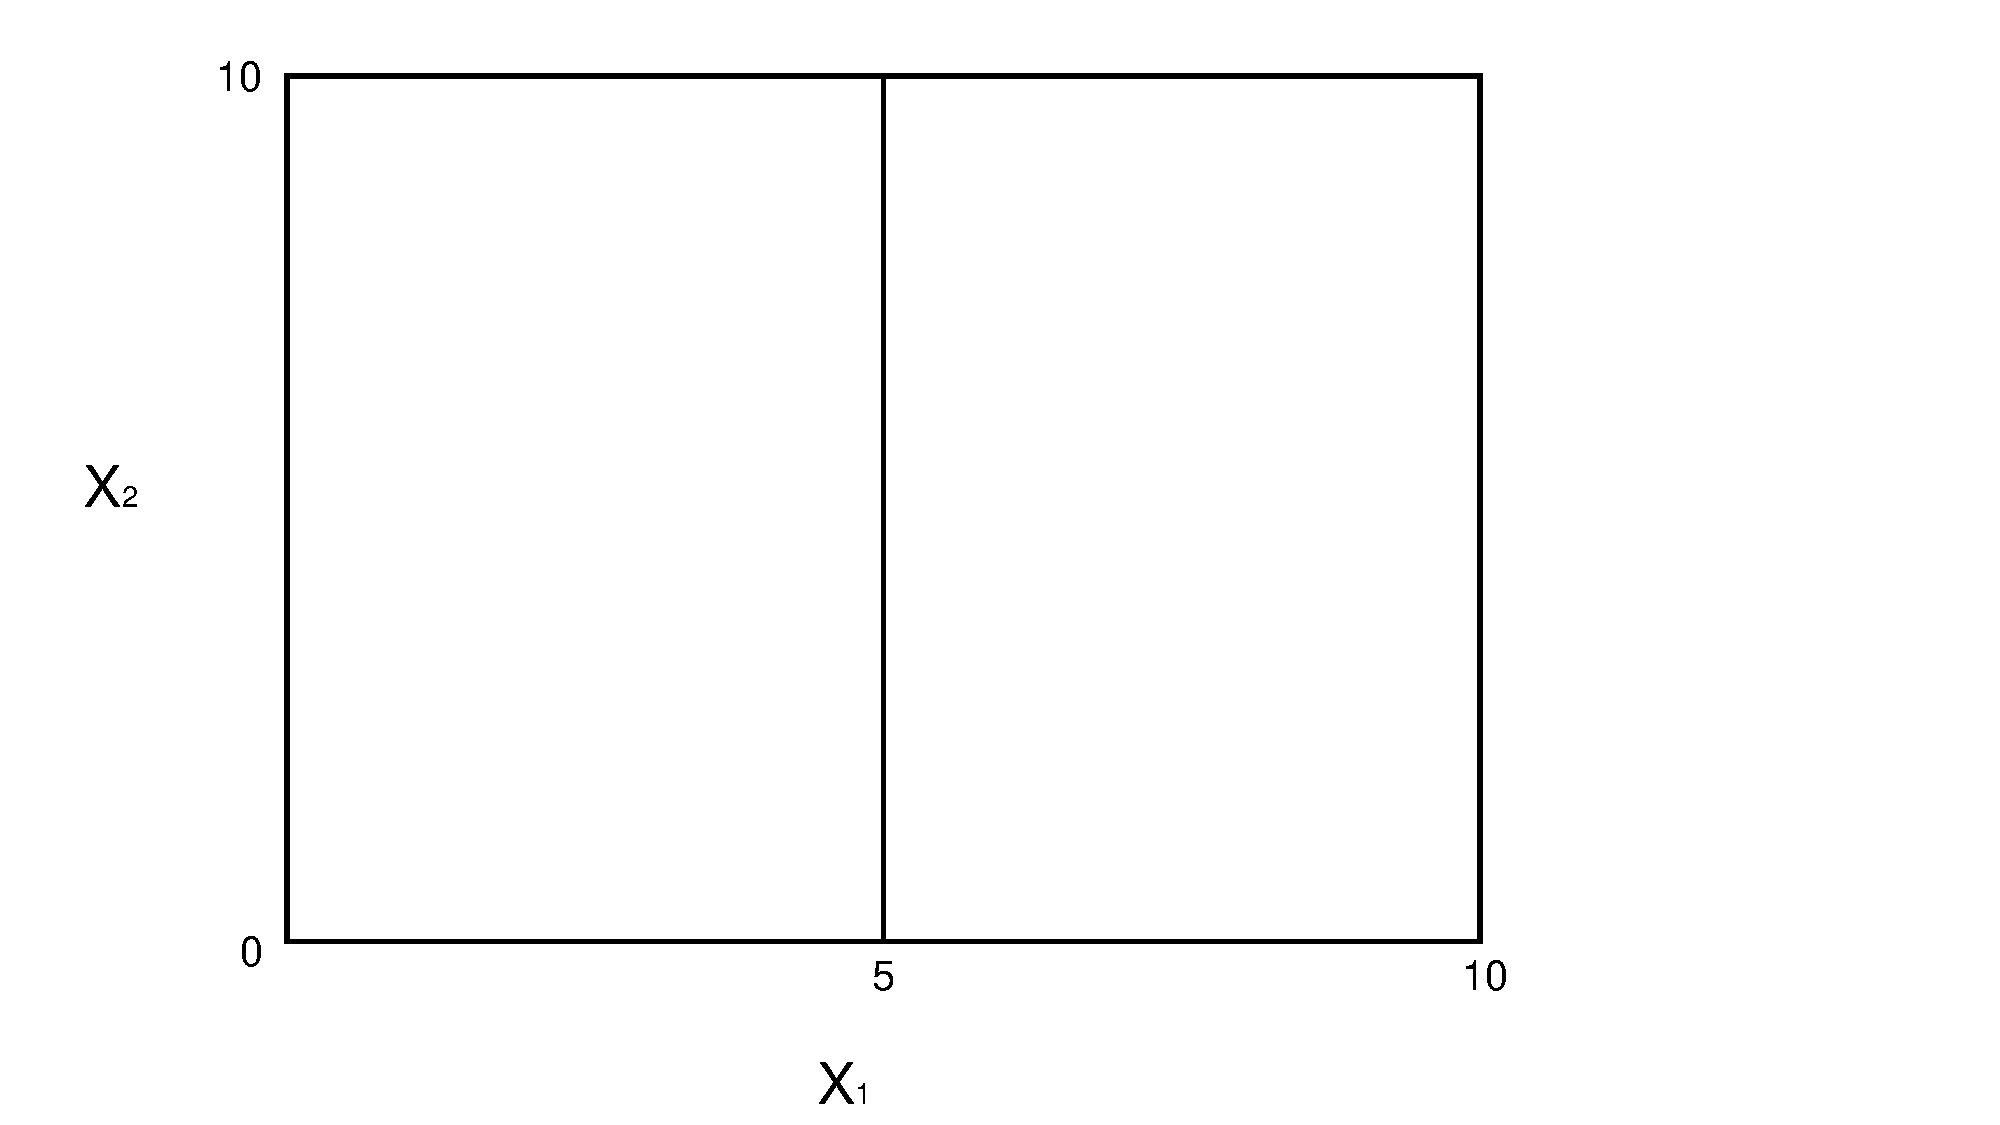
\includegraphics[scale=0.22]{P1b.pdf}
\end{figure}

\textit{The second split, $X_2<7$, partitions the left region further:}
\begin{figure}[!h]
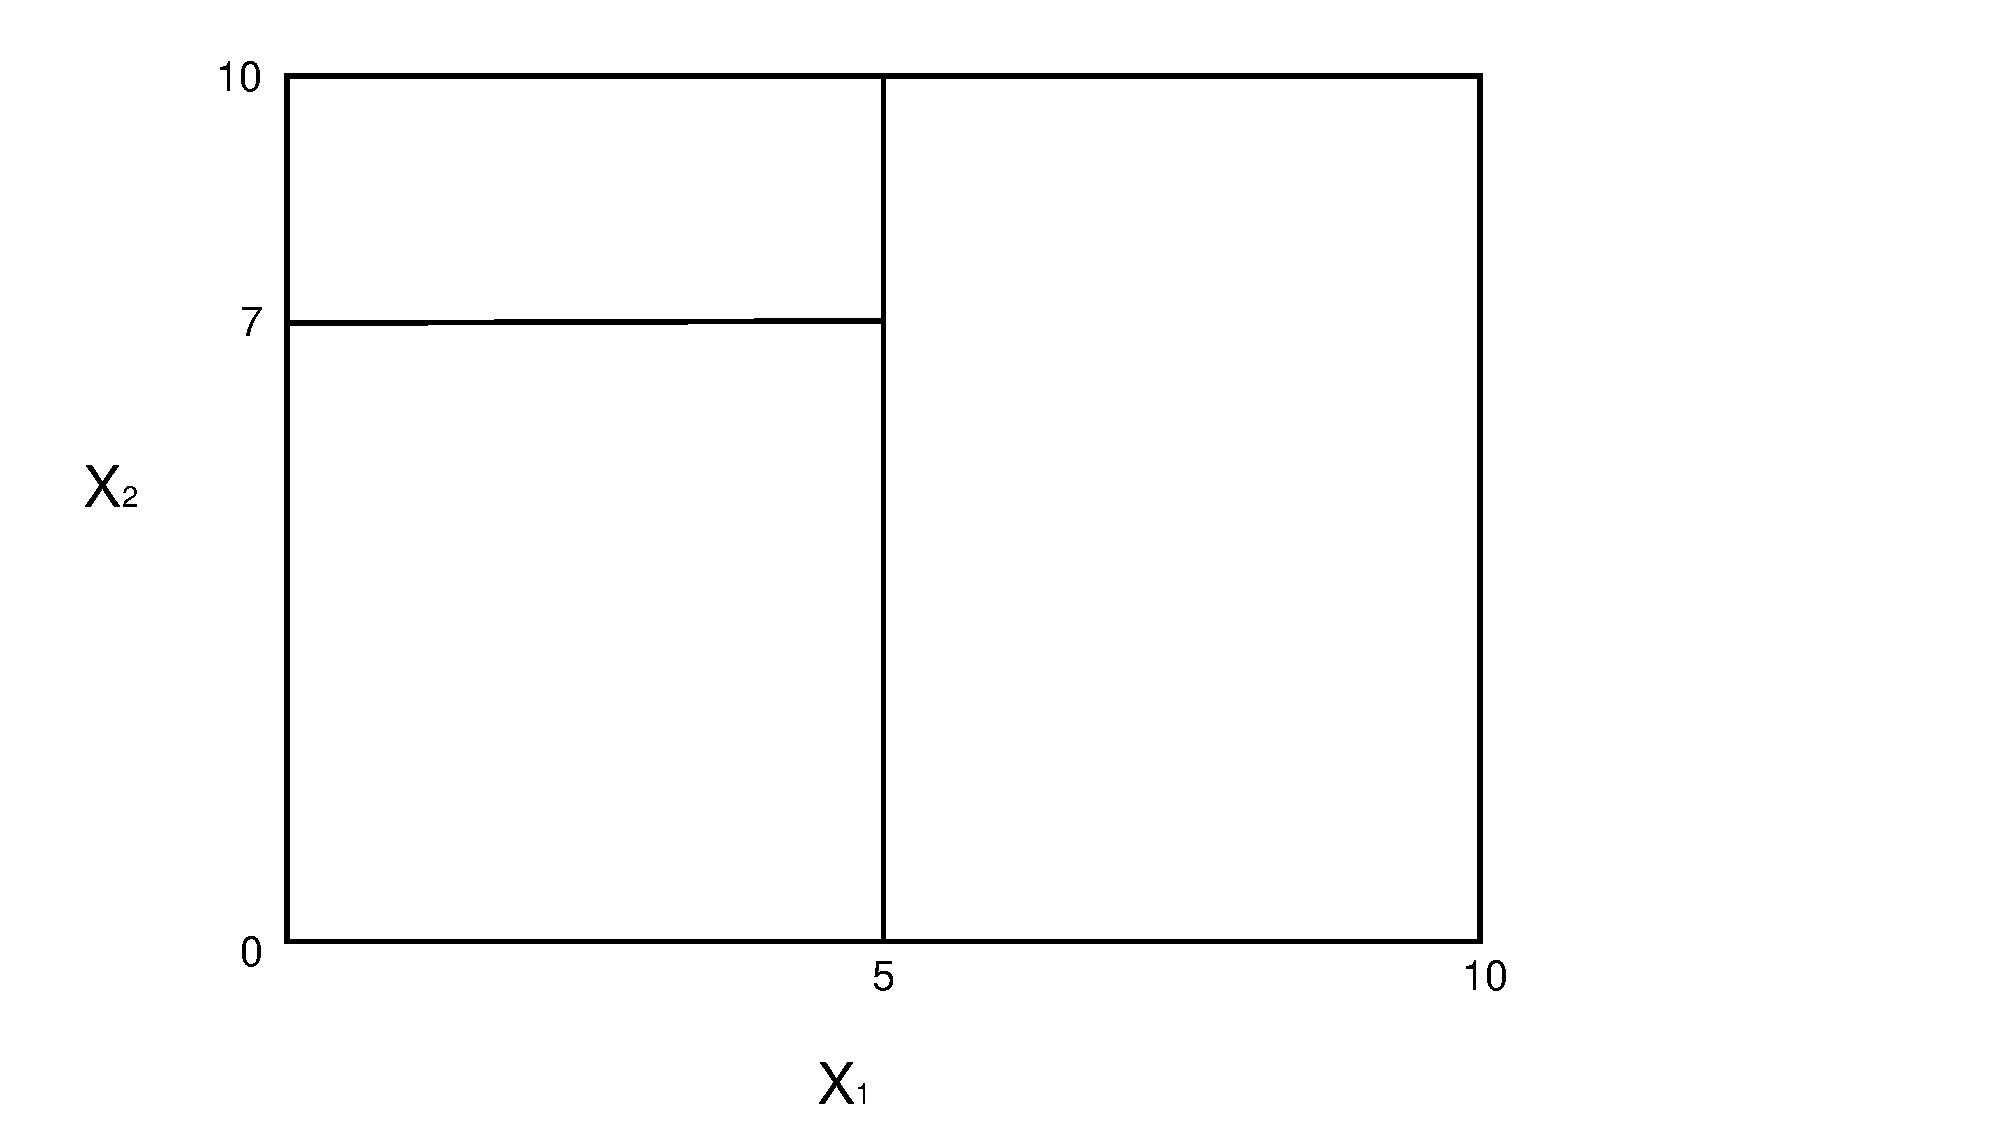
\includegraphics[scale=0.22]{P1c.pdf}
\end{figure}

\textit{Adding the constant predictions to the corresponding regions, we get the final solution:}
\begin{figure}[!h]
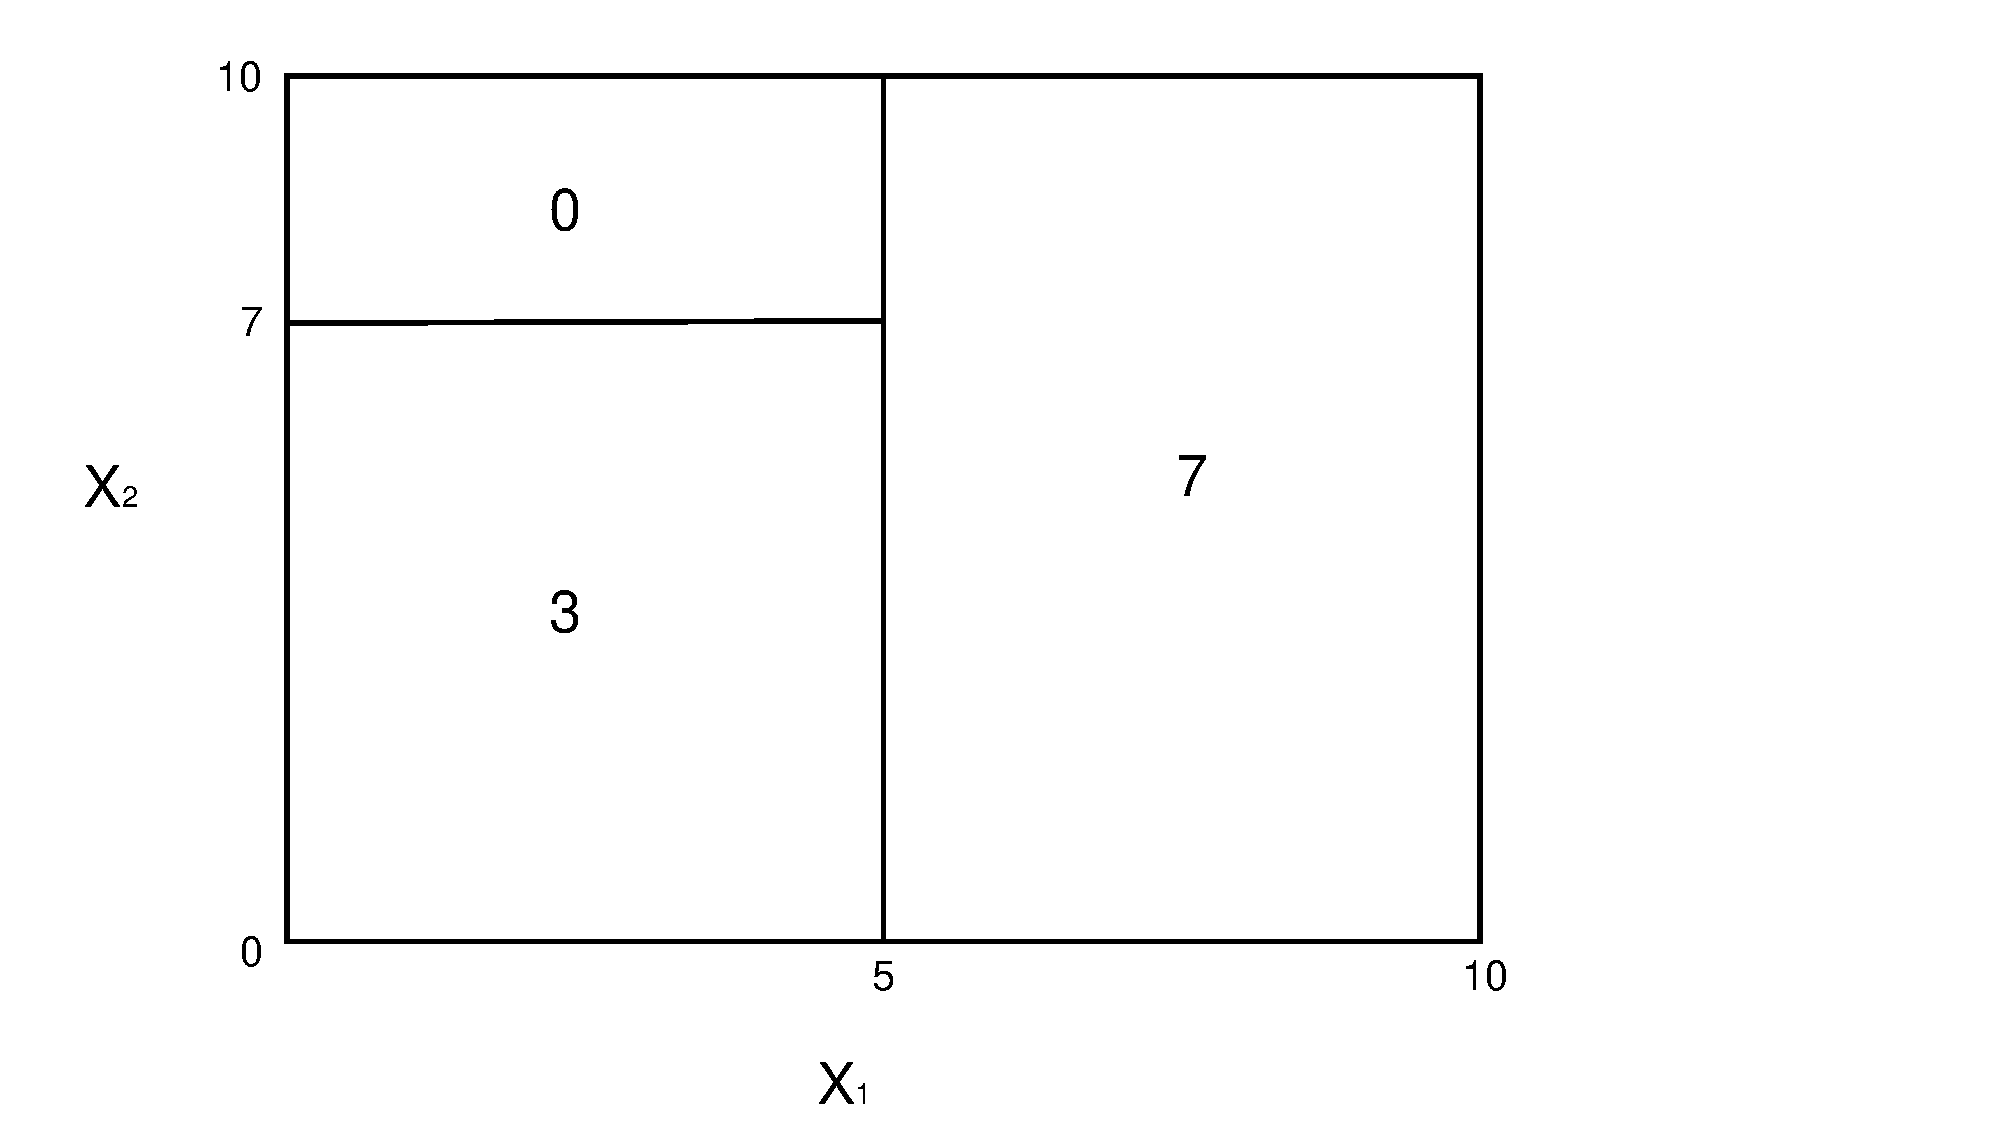
\includegraphics[scale=0.28]{P1.pdf}
\end{figure}

\clearpage

\textbf{(b)} \textit{Note that the partition results from the following two splits:}

\textit{First, the split $X_2<3$:}
\begin{figure}[!h]
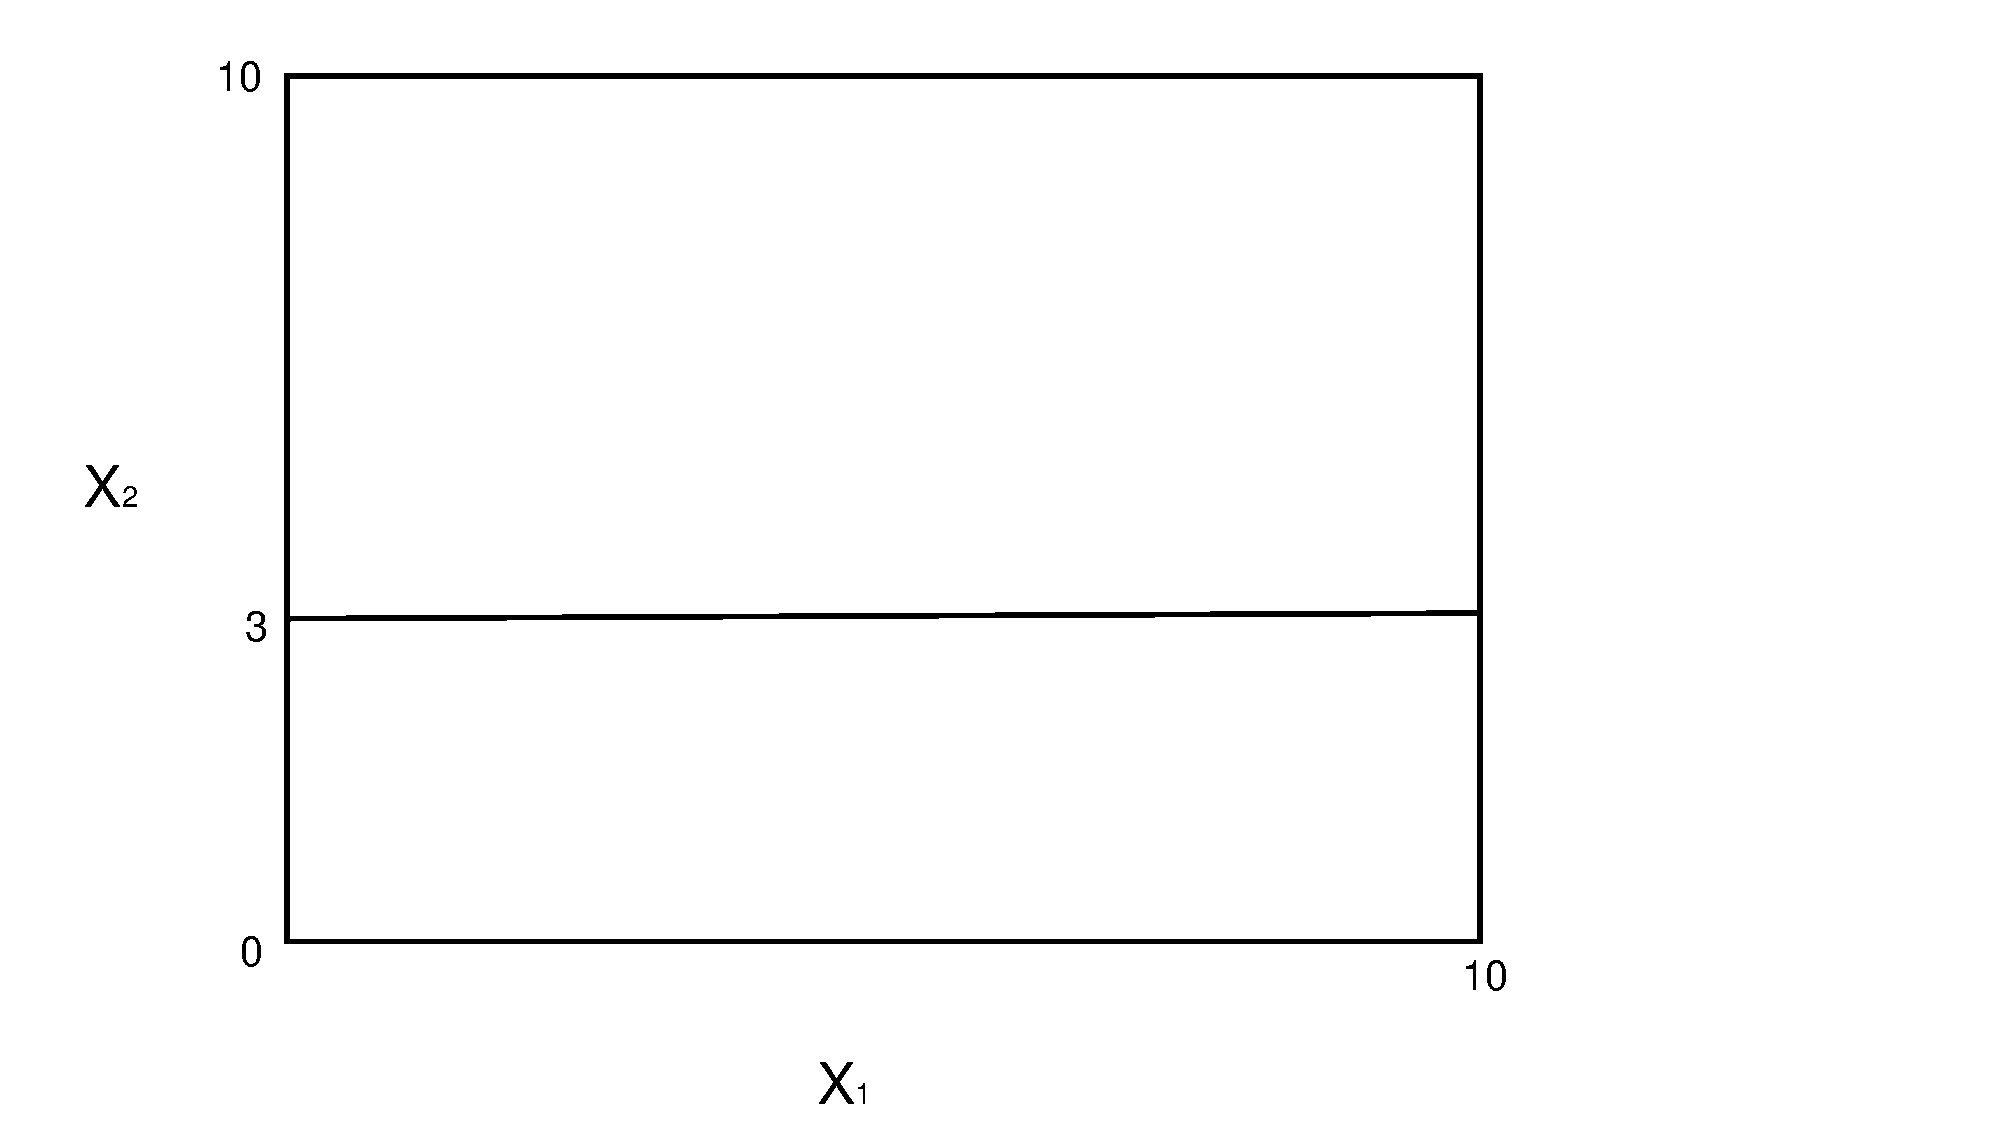
\includegraphics[scale=0.22]{P2b.pdf}
\end{figure}

\textit{Second, the split $X_1<4$, applied to the (top) region $X_2\ge 3$:}
\begin{figure}[!h]
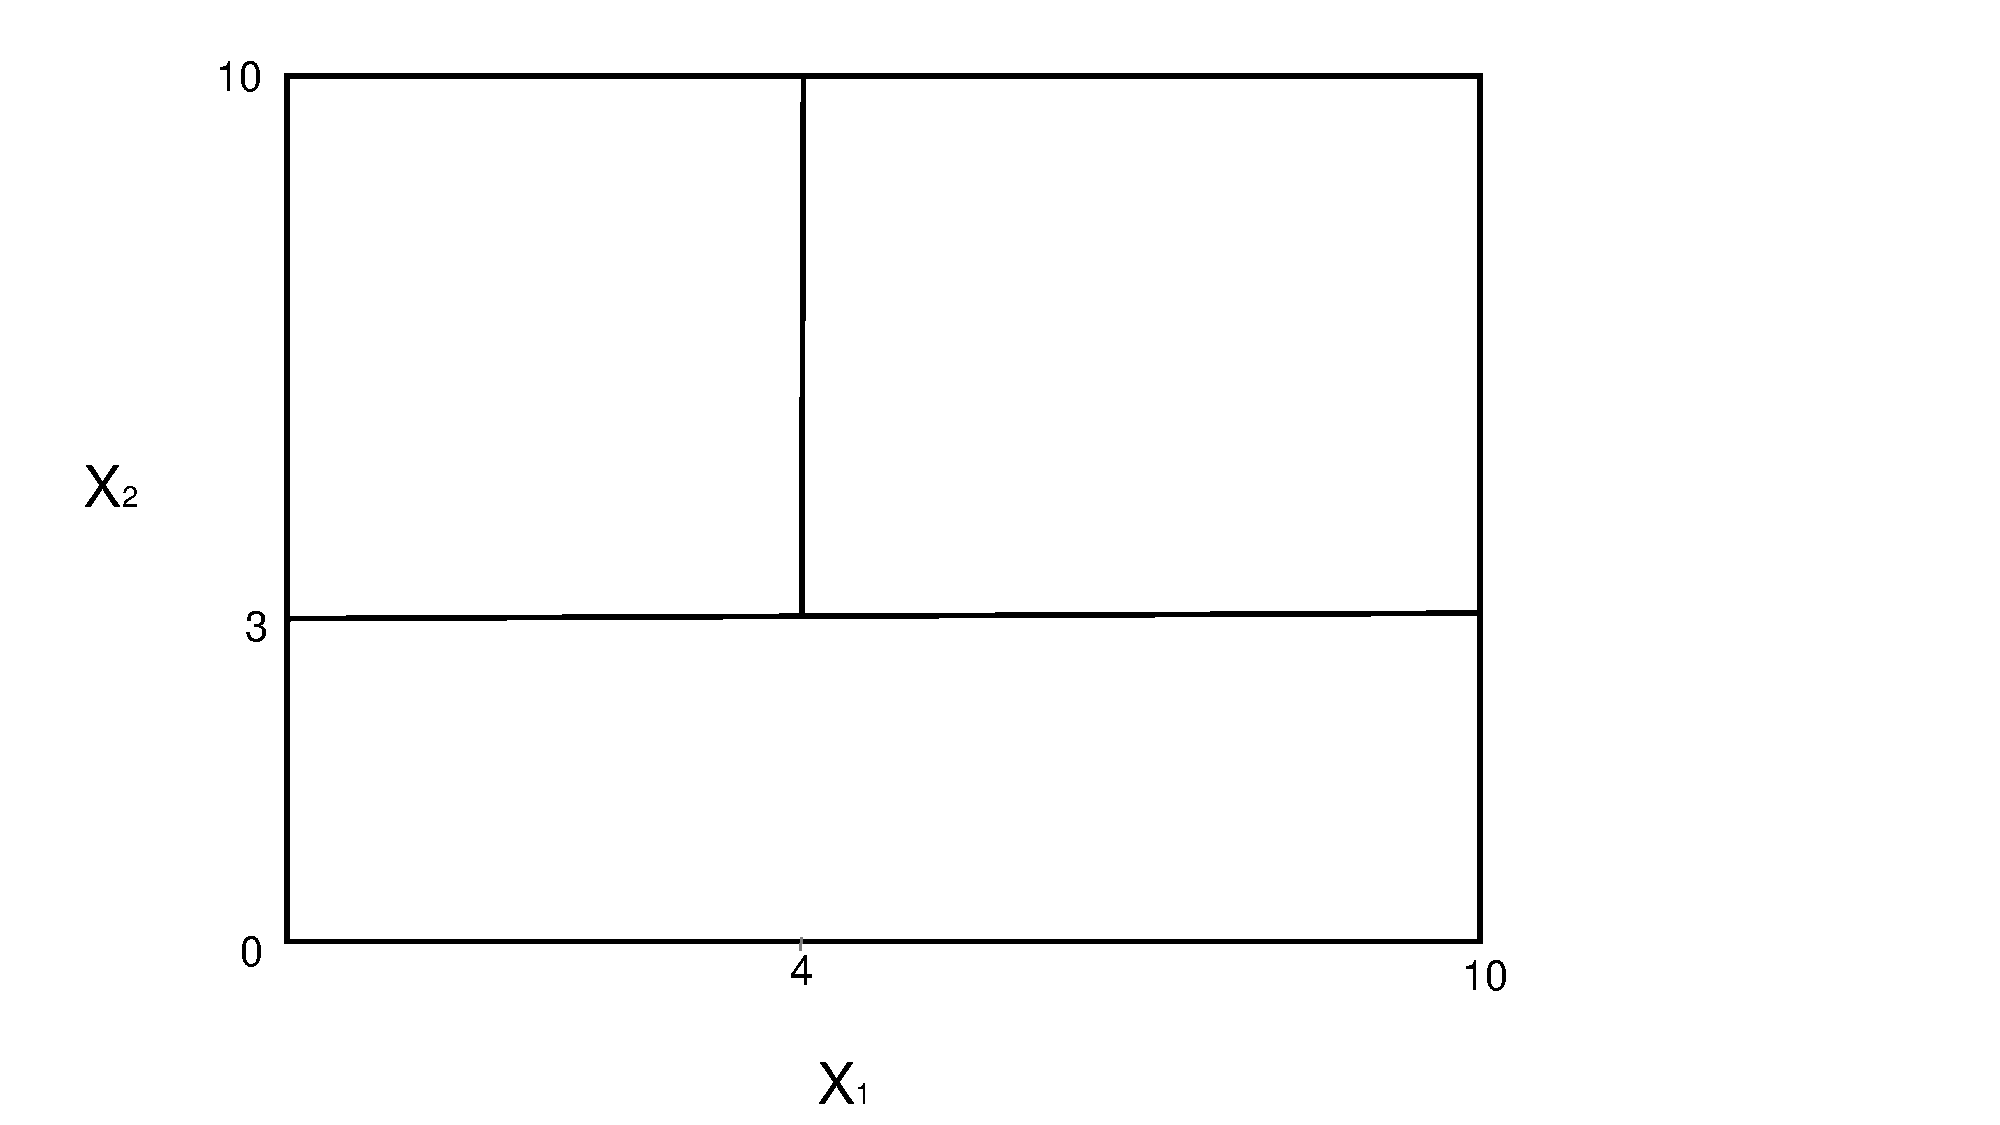
\includegraphics[scale=0.22]{P2c.pdf}
\end{figure}

Thus, the corresponding tree is:
\begin{figure}[!h]
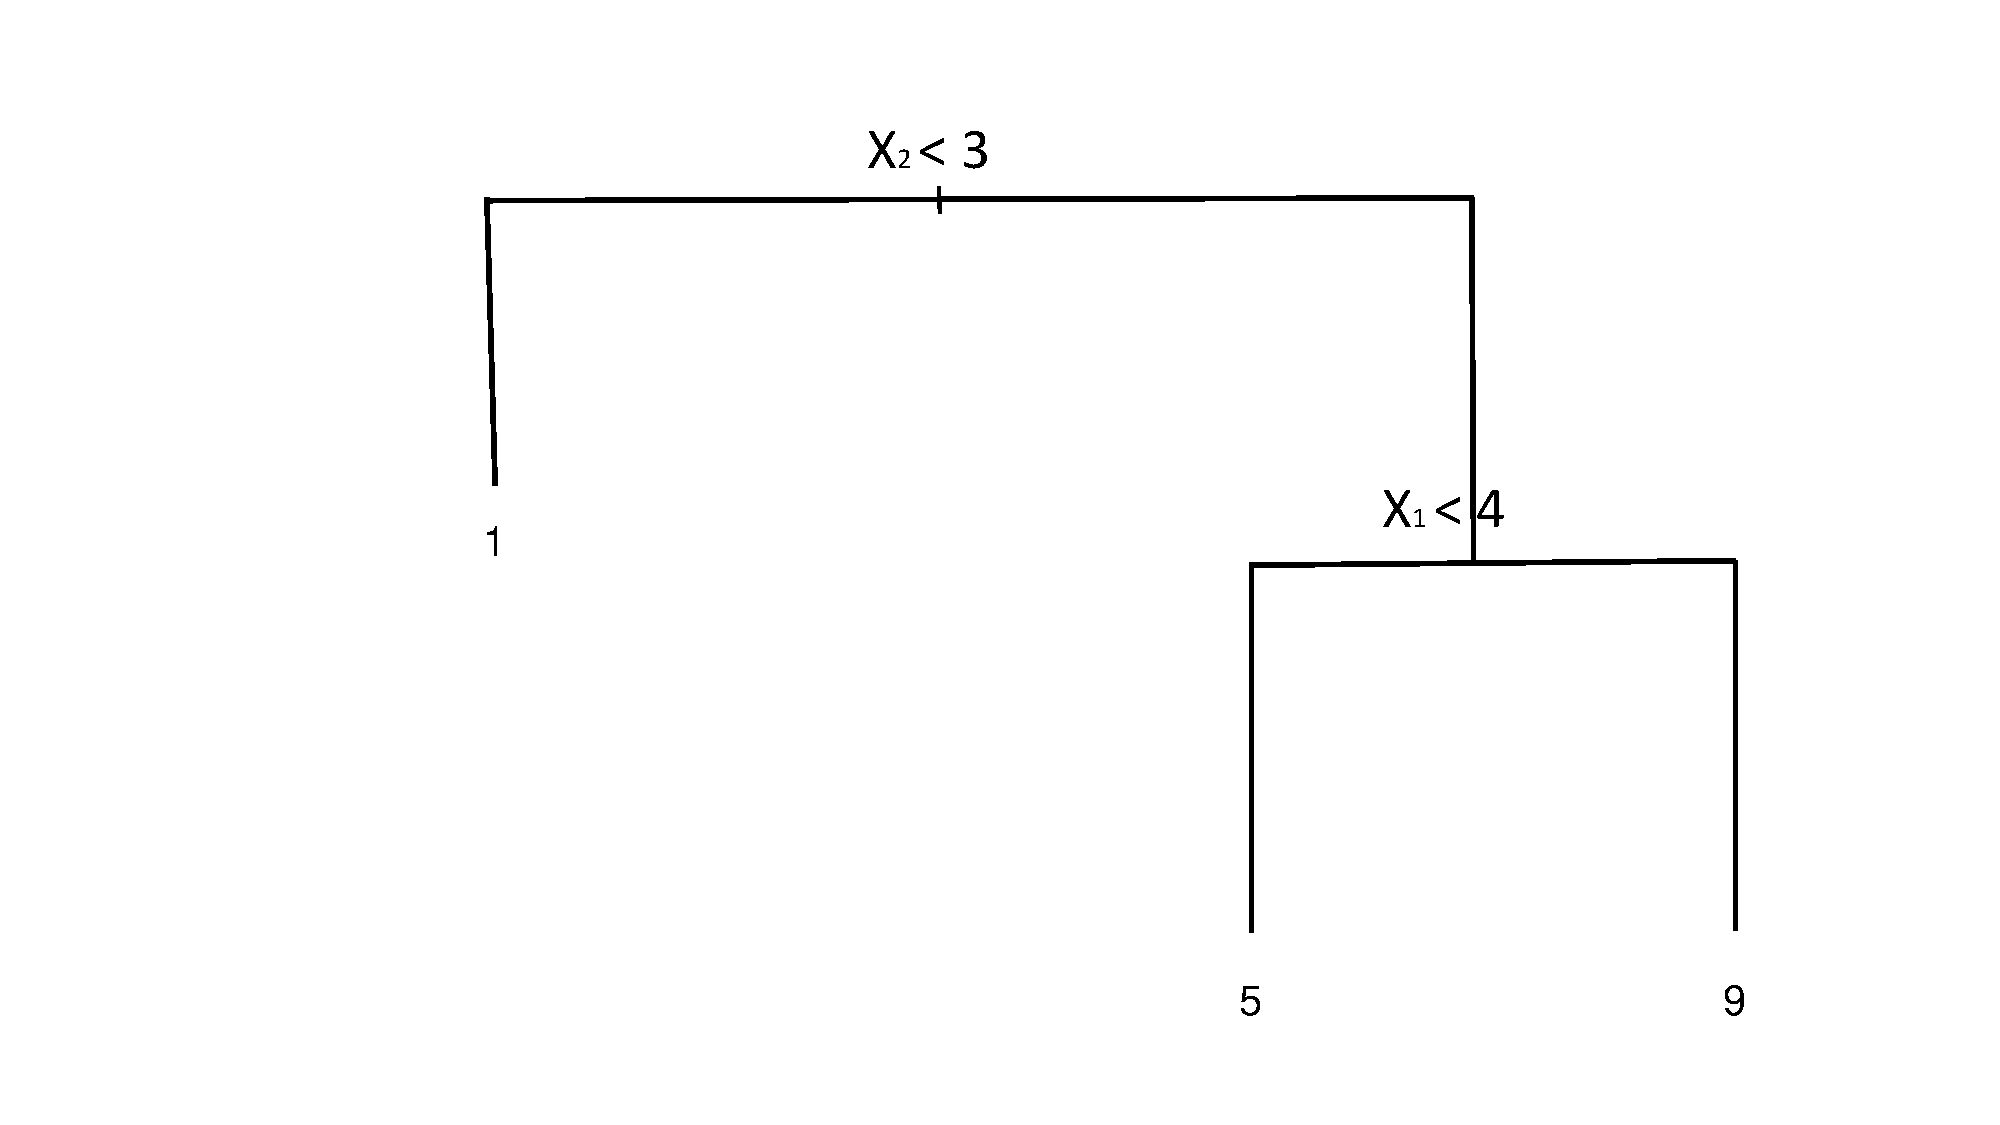
\includegraphics[scale=0.35]{T2.pdf}
\end{figure}

\textbf{(c)} \textit{The regression function corresponding to the tree above is :}
\begin{equation*}
\widehat{f}(x_1,x_2)=I\{x_2<3\}+5I\{x_2\ge3, x_1<4\}+9I\{x_2\ge3, x_1>4\}.
\end{equation*}
\textit{It corresponds to a nonlinear interaction model.  Note that a GAM regression function would have the general form $f(x_1,x_2)=f_1(x_1)+f_2(x_2)$.}


\end{document} 